\chapter{\IfLanguageName{dutch}{Resultaten van de proef}{Results of the test}}
\label{ch:resultaten}

\section[Onderzoeksvraag 1]{Onderzoeksvraag 1: Kan een (betere) onboarding en in-app user training ervoor zorgen dat de eindgebruiker een beter inzicht heeft op de totale functionaliteit van een grote applicatie?}
\label{sec:onderzoeksvraag-1}

Om een antwoord te formuleren op de eerste onderzoeksvraag kan men een aantal afhankelijke variabelen in overweging nemen. Enerzijds kan men kijken naar alle tijden op de zes taken, anderzijds naar de SUS-score en de vragen met betrekking tot learnability uit de SUS-vragenlijst, maar men kan ook in overweging nemen of de participant al dan niet om hulp vroeg tijdens één van de taken.

Deze laatste variabelen, namelijk de zes dichotome hulp-gevraagd variabelen, werden onderzocht met behulp van een $\chi^2$-test (chi-kwadraattest). In deze test werd de groep waarvan de participant deel uitmaakt als onafhankelijke variabele opgenomen. De resultaten zijn waar te nemen in tabel~\ref{tab:chisq-hulp}. Voor de opdrachten \textit{instellingen}, \textit{spaardoel toevoegen}, \textit{bedrag toevoegen} en \textit{berekening} hebben alle participanten het doel bereikt zonder hulp.

\begin{table}[]
    \centering
    \begin{tabular}{r|cccc}
        & $\chi^2$ & $df$ & $p$ & $N$ \\ \hline
        Spaardoel verwijderen & $5.16$ & $1$ & $0.02$ & $25$ \\
        Groot bedrag toevoegen & $0.003$ & $1$ & $0.95$ & $25$
    \end{tabular}
    \caption{$\chi^2$ resultaten indien de participant hulp nodig had}
    \label{tab:chisq-hulp}
\end{table}

Uit de resultaten van de $\chi^2$-test valt af te leiden dat er een significant verband is tussen de twee variabelen bij de opdracht \textit{spaardoel verwijderen}, $\chi^2 (1, N = 25) = 5.16$, $p = 0.02$, maar niet bij de opdracht \textit{groot bedrag toevoegen}, $\chi^2 (1, N = 25) = 0.003$, $p = 0.95$, $ns$. Bij enkele functionaliteiten zal de gebruiker dus minder hulp nodig hebben wanneer men bepaalde vormen van onboarding implementeert in de applicatie. Echter zal de gebruiker niet bij elke functionaliteit een voordeel halen uit de onboarding. Om te weten wanneer de onboarding van pas komt kan men best de applicatie laten testen door enkele personen en noteren waar deze problemen ondervinden.

Om de overige afhankelijke variabelen op te nemen in de analyses, werd eerst een $t$-test uitgevoerd. In deze $t$-test werd opnieuw als onafhankelijke variabele de groep waarvan de participant deel uitmaakt opgenomen. Als afhankelijke variabele werd gekozen voor een gemiddelde van de tijden op alle taken. Participanten voltooiden de opdrachten sneller wanneer deze de proof-of-concept applicatie hadden waarbij de onboarding en help-elementen beschikbaar waren ($M = 23.36$, $SD = 9.95$) in vergelijking met wanneer deze geen onboarding en help-elementen ter beschikking hadden ($M = 43.57$, $SD = 21.76$), $t(24.033) = -8.426$, $p < .001$.

Deze analyse toont een verschil aan tussen wanneer men wel of geen gebruik kon maken van de learnability-elementen, maar de assumptie wordt gemaakt dat het effect van learnability-elementen op de zes taken gelijkaardig genoeg is dat er een gemiddelde van kan worden genomen. Omwille van deze reden wordt voor elke taak apart nog eens een $t$-test uitgevoerd. De resultaten van deze $t$-test zijn waar te nemen in tabel~\ref{tab:ttest-opdrachten}. Per opdracht is ook hier duidelijk dat participanten die gebruik maakten van onboarding en help-elementen significant minder tijd nodig hadden om de opdracht te voltooien. De gemiddelde tijden zijn te vinden in tabellen~\ref{tab:beschrijving-tijden-zonder-elementen} en \ref{tab:beschrijving-tijden-met-elementen}. De berekening van deze waarden in R is bijgevoegd in bijlage~\ref{bijlage:r-1}.

\begin{table}[]
	\centering
	\begin{tabular}{r|ccc}
		\textbf{Opdracht} & \textbf{$t$} & \textbf{$df$} & \textbf{$p$} \\ \hline
		Instellingen & $-8.55$ & $24.10$ & $< 0.001$ \\
		Spaardoel toevoegen & $-11.11$ & $24.04$ & $< 0.001$ \\
		Bedrag toevoegen & $-9.27$ & $24.05$ & $< 0.001$ \\
		Spaardoel verwijderen & $-4.19$ & $24.01$ & $< 0.001$ \\
		Berekening & $-10.55$ & $24.05$ & $< 0.001$ \\
		Groot bedrag toevoegen & $-5.27$ & $24.01$ & $< 0.001$ \\
		\textit{SUS-score} & $-29.36$ & $24.07$ & $< 0.001$
	\end{tabular}
	\caption{$t$-testen van alle opdrachten}
	\label{tab:ttest-opdrachten}
\end{table}

Een betere onboarding kan er zeker en vast voor zorgen dat de eindgebruiker sneller met de applicatie overweg kan. Hoe goed deze applicatie is in de ogen van de gebruiker hangt echter van meerdere variabelen af. Zo is een matige applicatie met een goede learnability niet rechtstreeks een betere applicatie. Waar en wanneer er in-app help elementen moeten geïmplementeerd worden hangt sterk af van de gebruiker. Wat vaak werd opgemerkt bij het afnemen van deze proef is dat elke gebruiker verschillend is en de ene gebruiker een bepaalde functionaliteit begrijpt zonder hulp terwijl de andere gebruiker sterk leunt op de hulp. Bij het bouwen van een applicatie moet dus zeker rekening gehouden worden met het doelpubliek bij het implementeren van onboarding en help-elementen. Usability tests voor en na die implementatie zijn sterk aan te raden voor betere inzichten.

\section[Onderzoeksvraag 2]{Onderzoeksvraag 2: Hoe een grote hoeveelheid aan functionaliteiten beheersbaar houden voor de eindgebruiker?}
\label{sec:onderzoeksvraag-2}

Het beheersbaar houden van een aanzienlijke hoeveelheid aan functionaliteiten is niet enkel een taak voor de onboarding en andere learnability elementen. Dit is een breder probleem waarvoor men idealiter een verder onderzoek in het \acrshort{acr:ux}-vakgebied houdt. Zoals in hoofdstuk~\ref{sec:learnability}, \ref{sec:onboarding} en \ref{sec:in-app-training} te lezen valt, is het voorzien van bepaalde onboarding en help-elementen wel een stap in de goede richting. Bij het afnemen van de proef viel ook op te merken dat voor de herhaling van de opdracht waar men een bedrag moest toevoegen de participant zelfverzekerder was wanneer deze de proof-of-concept applicatie had waarin de learnability-elementen aanwezig waren. Zo waren minder twijfels merkbaar.

Waarop zeker gefocust moet worden bij de implementatie van learnability-elementen in software van een aanzienlijke omvang is dat men de gebruiker initieel niet overspoelt met uitleg. De gebruiker verliest zo snel de aandacht en zal niet alles kunnen onthouden. Hotspots (zie hoofdstuk~\ref{sec:onboarding:hotspots}) zijn zo vaak een betere keuze dan een rondleiding (zie hoofdstuk~\ref{sec:onboarding:rondleidingen}), omdat de gebruiker zo zelf kiest wanneer deze wil starten met de uitleg.

Men kan de beheersbaarheid meten met de vragen uit de SUS-vragenlijst die betrekking hebben tot learnability. Participanten antwoorden gunstiger op deze vragen wanneer deze de proof-of-concept applicatie hadden waarbij de onboarding en help-elementen beschikbaar waren (vraag 4: $M = 1.31$, $SD = 0.85$, vraag 10: $M = 1.62$, $SD = 1.04$) in vergelijking met wanneer deze geen onboarding en help-elementen ter beschikking hadden (vraag 4: $M = 1.67$, $SD = 0.78$, vraag 10: $M = 1.83$, $SD = 0.83$), vraag 4: $t(40.07) = -4.96$, $p < .001$, vraag 10: $t(37.09) = -5.63$, $p < .001$. De berekening van deze waarden in R is bijgevoegd in bijlage~\ref{bijlage:r-2}.

\section[Onderzoeksvraag 3]{Onderzoeksvraag 3: Heeft (het gebrek aan) in-app user training effect op de gebruiksduur en/of levensduur van de applicatie?}
\label{sec:onderzoeksvraag-3}

Indien de gebruiker de applicatie voor een langdurige periode zou gebruiken is moeilijk te voorspellen. De belangrijkste fase voor de gebruiksduur is het initieel gebruik. Wanneer de gebruiker niet overtuigd is van de applicatie zal hij of zij die sneller terug verwijderen. Als afsluitende vraag in de proef werd aan de participanten gevraagd indien ze deze applicatie zouden houden op hun toestel of indien ze deze zouden verwijderen of vergelijken met concurrerende software.

In figuur~\ref{fig:beschrijving-would-keep} is te merken dat er eventueel een verschil zal zijn tussen de groep met en zonder onboarding en usability elementen. Na uitvoering van de $\chi^2$-test is er echter geen significante relatie merkbaar tussen het al dan niet aanwezig zijn van learnability-elementen en indien de participant de applicatie zou houden op zijn of haar persoonlijk toestel, $\chi^2 (1, N = 25) = 1.92$, $p = 0.17$, $ns$. De gebruiker die toegang had tot onboarding en help-elementen was dus niet meer geneigd de applicatie te houden dan de gebruiker die hiertoe geen toegang had. Een verklaring hiervoor kan zijn dat een hele hoop meer factoren hierop inspelen. Deze proef is bijvoorbeeld uitgevoerd bij participanten waarvan niet iedereen op zoek was naar een applicatie met deze functionaliteit De berekening van deze waarden in R is bijgevoegd in bijlage~\ref{bijlage:r-3}.

\section[Onderzoeksvraag 4]{Onderzoeksvraag 4: Hoe de eindgebruiker wegwijs maken in een grote applicatie?}
\label{sec:onderzoeksvraag-4}

Hoe een gebruiker omgaat met de functionaliteiten binnen de applicatie is één ding, maar de gebruiker moet uiteraard ook overweg kunnen met de navigatie binnen deze applicatie om zo bij de gewenste functionaliteiten uit te komen. Net zoals bij onderzoeksvraag 2 (zie hoofdstuk~\ref{sec:onderzoeksvraag-2}) is dit een breder probleem uit het \acrshort{acr:ux}-vakgebied. Participanten uit deze proef hebben wel aangetoond dat deze het handig en bruikbaar vonden dat bij de initiële opstart van de applicatie er een uitleg was voorzien voor de elementen in de tab-bar (zie figuur~\ref{fig:piggy:tabbar}). Een uitleg voorzien zorgt ervoor dat de iconen uit de navigatie een duidelijke betekenis krijgen. Hierdoor gaat de navigatie vlotter.

\begin{figure}[h!]
    \centering
    
\includegraphics[width=.5\columnwidth]{piggy-tabbar}
    \caption{Navigatie in de proof-of-concept applicatie}
    \label{fig:piggy:tabbar}
\end{figure}

Om de gebruiker niet aan zijn of haar lot over te laten is het mogelijk om deze in de onboarding al enkele taken te laten voltooien vooraleer aan het echte werk te beginnen. In de proof-of-concept applicatie was het mogelijk om een naam in te stellen, dit kon zowel in de instellingen als in de onboarding (zie figuur~\ref{fig:piggy:name}). In de proef viel op dat enkel participanten die de proof-of-concept applicatie met onboarding hadden de naam ook effectief wijzigden (zie figuur~\ref{fig:beschrijving-changed-name}).

\begin{figure}[h!]
	\centering
	\subfloat[Instellingen]{
		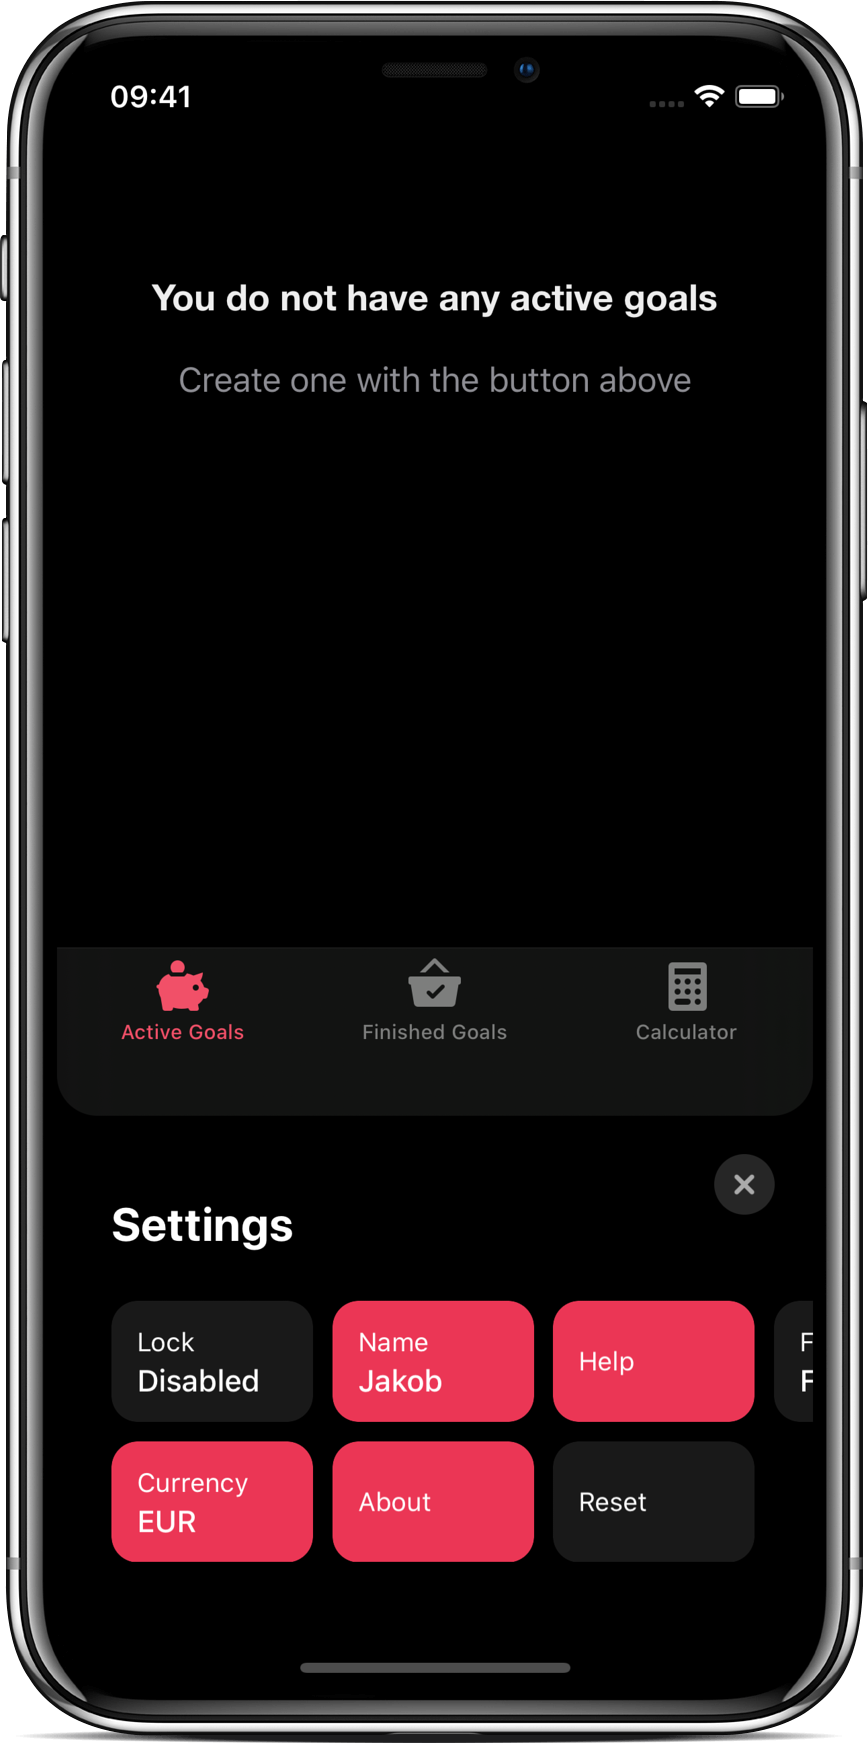
\includegraphics[width=.27\linewidth]{piggy-name-settings-1}
		\label{fig:piggy:name:settings}
	}
	\qquad
	\subfloat[Naam wijzigen in instellingen]{
		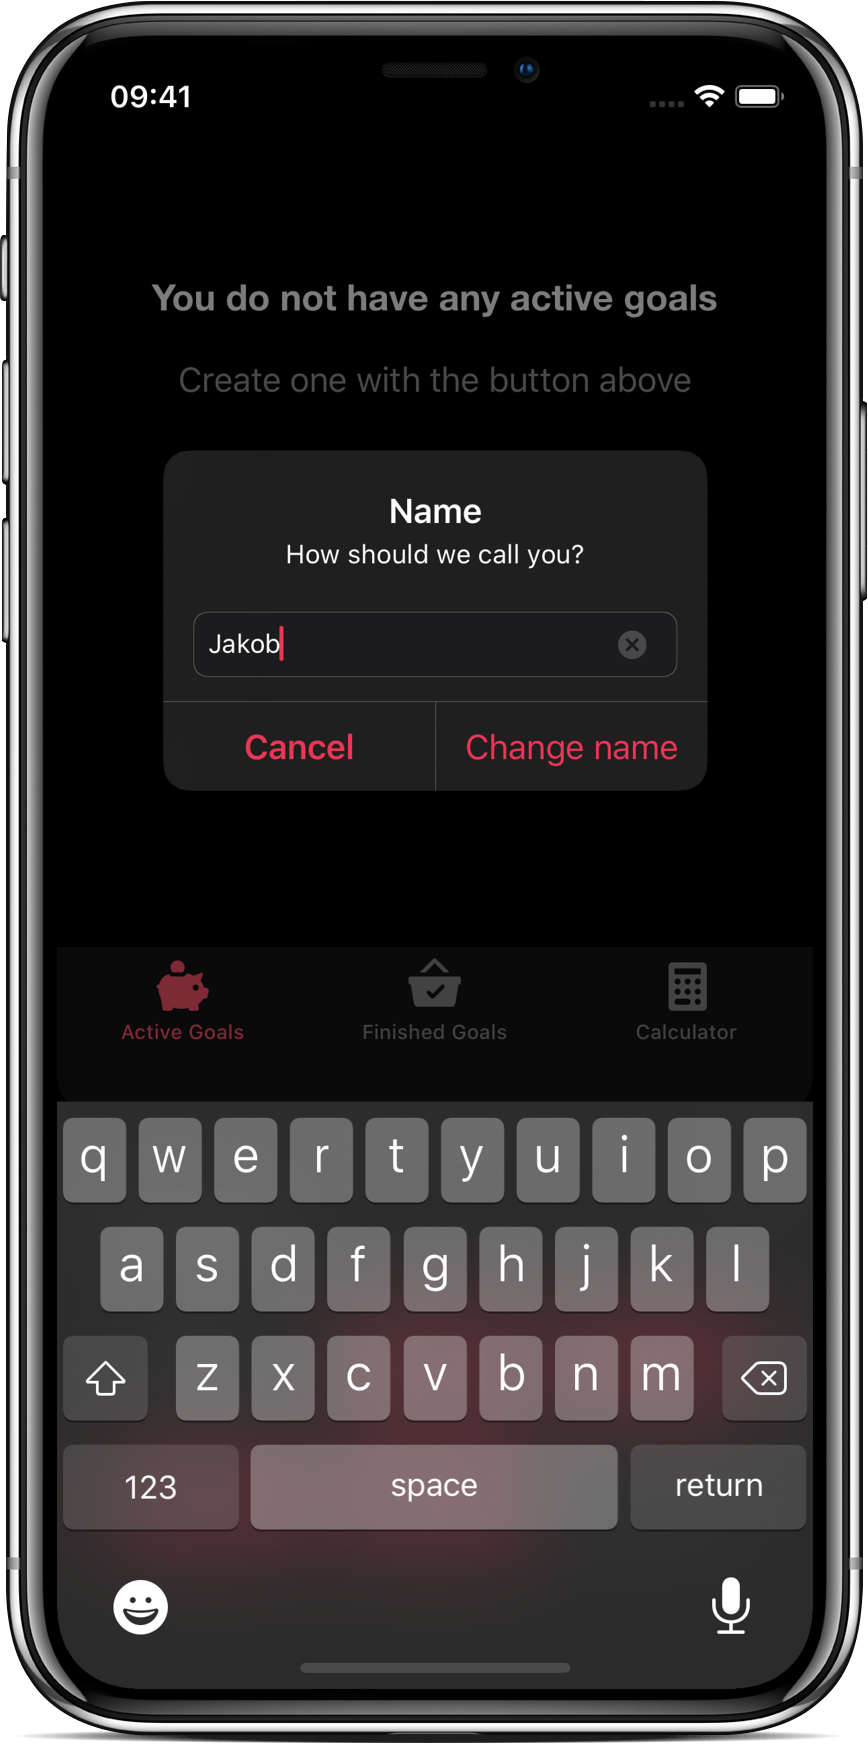
\includegraphics[width=.27\linewidth]{piggy-name-settings-2}
		\label{fig:piggy:name:settings-2}
	}
	\qquad
	\subfloat[Naam wijzigigen in onboarding]{
		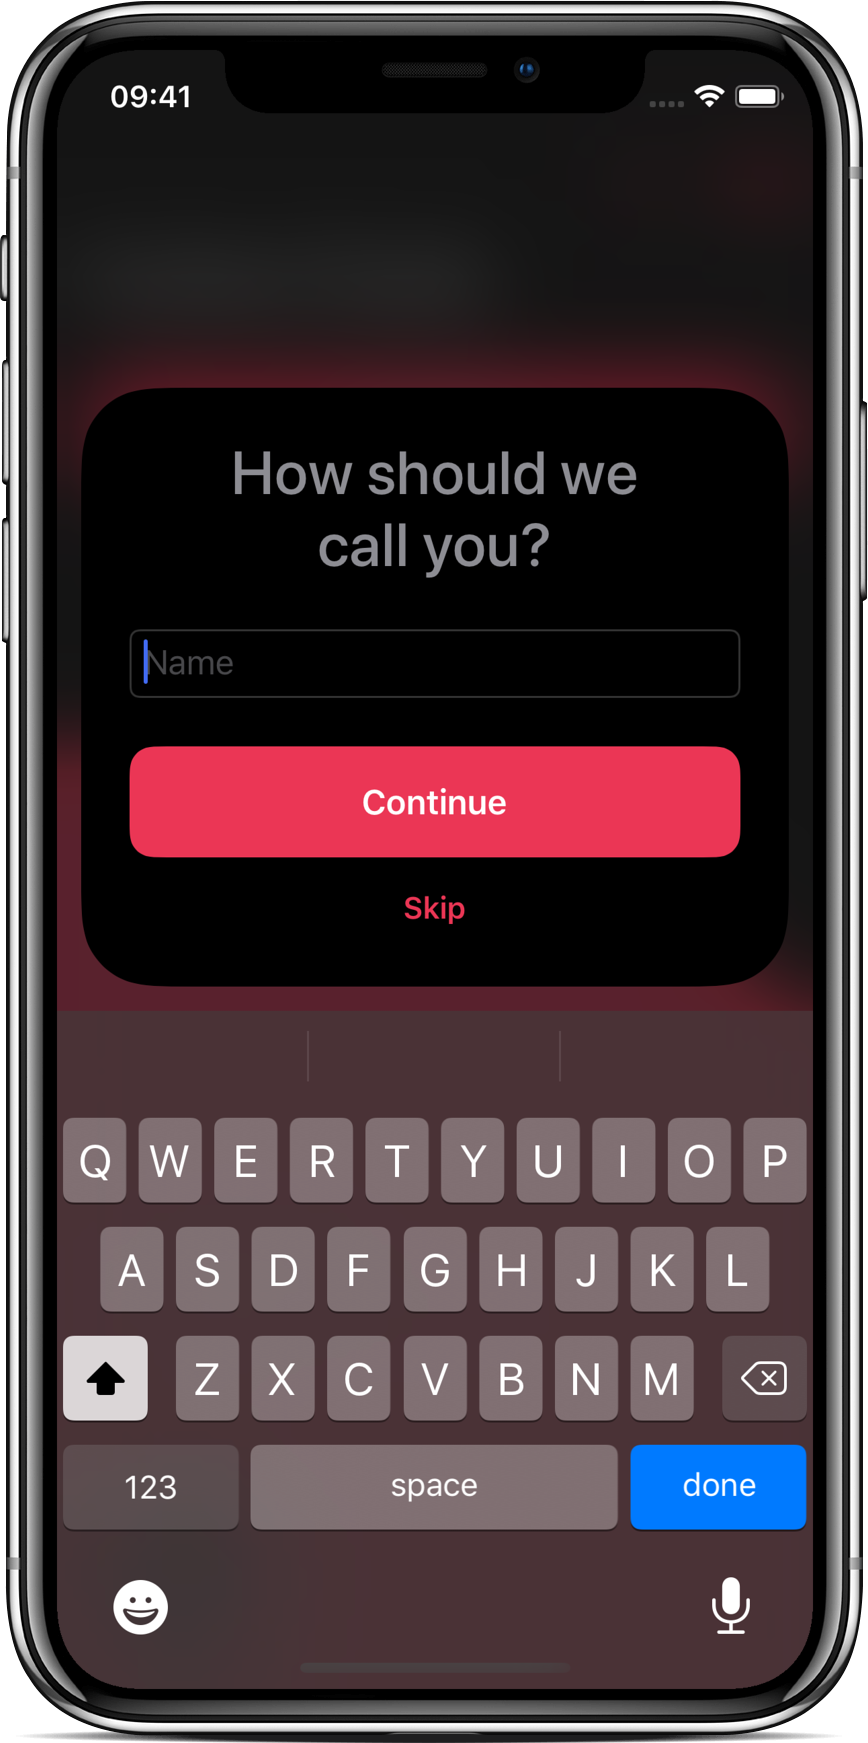
\includegraphics[width=.27\linewidth]{piggy-name-onboarding}
		\label{fig:piggy:name:onboarding}
	}
	\caption{De naam van de gebruiker wijzigen in de proof-of-concept applicatie}
	\label{fig:piggy:name}
\end{figure}

\begin{figure}[h]
	\centering
	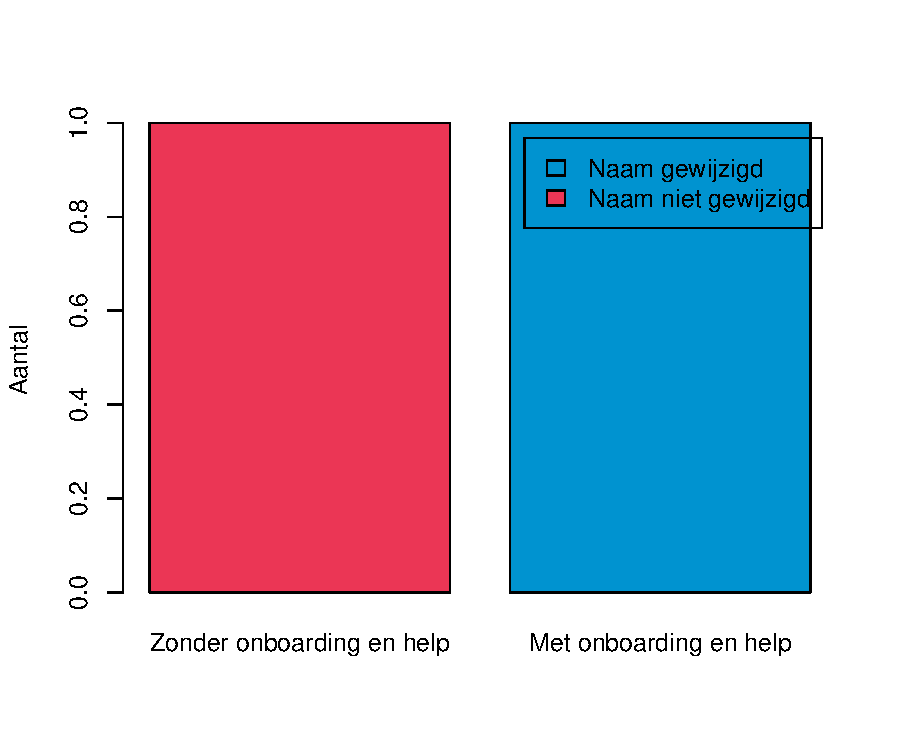
\includegraphics[width=.46\columnwidth]{beschrijving-changed-name}
	\caption{Indien de participant de naam wijzigde bij het verkennen van de applicatie}
	\label{fig:beschrijving-changed-name}
\end{figure}
